\chapter{Numerical Model and CFD Setup}
\label{ch:numerical_setup}

This chapter provides an overview of the physical and computational setup employed for the fluid dynamic simulation of the excess flow valves. The discussion covers the governing equations, fluid property modeling, boundary condition architecture, hardware and software HPC environment, hybrid grid generation pipeline, parallel domain decomposition, and solver troubleshooting within OpenFOAM \cite{openfoam_user}. %

\section{Governing Equations, Turbulence Modeling and Physical properties}
\label{sec:governing_equations}
The fluid modelled to simulate the valves is assumed to be both steady-state and incompressible, so underlying implicitly that the gas flows with a Mach number which remains below the compressibility threshold of $Ma < 0.3$ \cite{anderson2017} allowing the fluid density $\rho$ to be treated as constant. Consequently, the governing Reynolds-Averaged Navier-Stokes (RANS) equations for conservation of mass (continuity) and momentum reduce to their kinematic forms \cite{white2016, moukalled2016}:

\begin{equation}
    \nabla \cdot \mathbf{U} = 0
    \label{eq:continuity}
\end{equation}

\begin{equation}
    \nabla \cdot (\mathbf{U} \otimes \mathbf{U}) = -\nabla P + \nabla \cdot \left[ (\nu + \nu_t) \left( \nabla \mathbf{U} + (\nabla \mathbf{U})^T \right) \right]
    \label{eq:momentum}
\end{equation}

\vspace{0.8mm}

where $\mathbf{U}$ is the Reynolds-averaged velocity vector, $P = p/\rho$ is the kinematic pressure (static pressure divided by density, with dimensions $[\text{m}^2/\text{s}^2]$), $\nu = \mu/\rho$ is the molecular kinematic viscosity, and $\nu_t$ is the turbulent eddy kinematic viscosity \cite{openfoam_user, moukalled2016}.
\newline \\
To close the RANS system and accurately resolve both the near-wall boundary layer along the valve casing and the detached shear layers downstream of the obturator orifices, the two-equation $k-\omega$ Shear Stress Transport (SST) turbulence model \cite{menter1994} has been employed. This model has been chosen because it blends the $k-\omega$ model in the viscous near-wall region with the freestream-independent $k-\epsilon$ model in the bulk flow, providing better accuracy in adverse pressure gradients and separating flows, which are expected in a complex geometry like the tested valves channels.

In OpenFOAM the solved RANS system is divided by density $\rho$, so to characterize the working fluid from a transport perspective, only the kinematic viscosity $\nu$ is needed \cite{openfoam_user}. In OpenFOAM 10, this property ha to be specified inside the \texttt{constant/physicalProperties} dictionary using the constant viscosity model \cite{openfoam_user}: %

\vspace{1.5mm}

\begin{lstlisting}[language=C++, captionpos=b, caption={Structure of the \texttt{constant/physicalProperties} dictionary.}]
viscosityModel  constant;

nu              [0 2 -1 0 0 0 0] NU_VALUE;
\end{lstlisting} %

Here, the dimensional set \texttt{[0 2 -1 0 0 0 0]} enforces SI units of $\text{m}^2/\text{s}$ in the [\textit{kg m s K mol A cd}] system, and \texttt{NU\_VALUE} acts as a parameter for automated injection during the Design of Experiments. 

\section{Domain geometry and Boundary Conditions}
\label{sec:boundary_conditions}
The numerical domain that represents the different valve solutions has been divided into 5 different sections in order to create a modular system for the DoE building and applying different boundary conditions together with different meshing parameters. Moreover, this is useful for further data post processing, splitting the simulation outputs on different domain zones.

\begin{figure}[H]
    \centering
    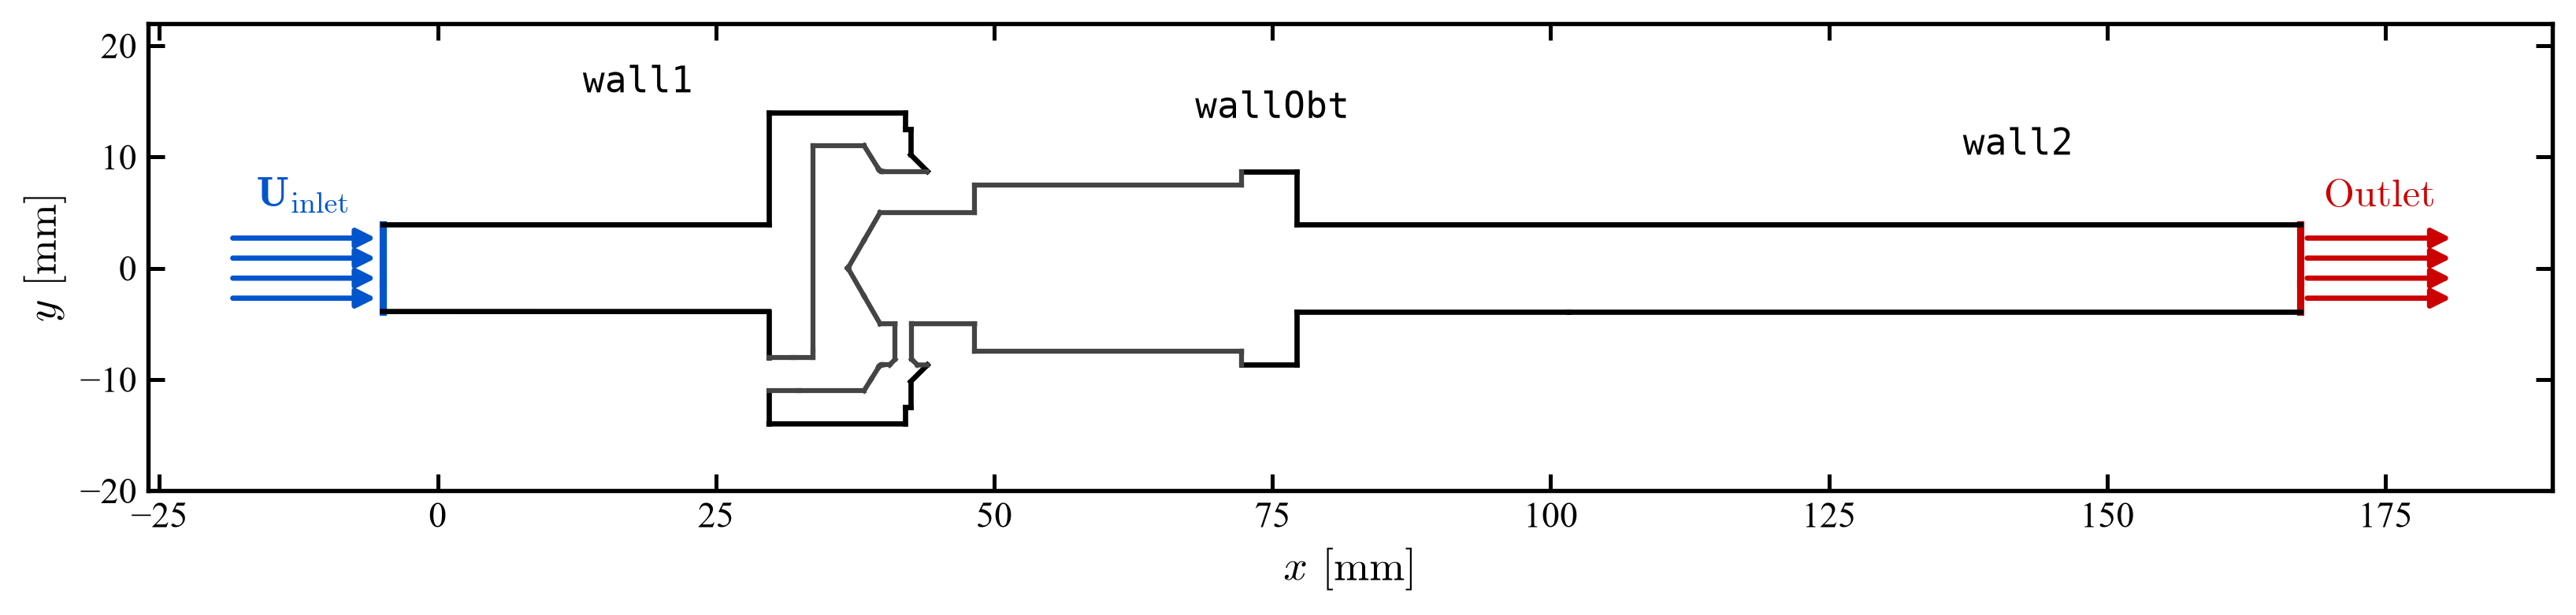
\includegraphics[scale=0.5]{Pics/Slice_ObtA.png}
    \caption{Slice of the numerical domain}
    \label{fig:dominio}
\end{figure}

The \ref{fig:dominio} shows the different domain sections, also highlighting the direction of the fluid flowing inside the valve. The geometry has the inlet and outlet not positioned right near the obturator to avoid numericla errors and not having at the inlet an inlfuence of the outlet boundary condition.

\begin{table}[H]
\centering
\label{tab:domainBC}
\begin{tabular}{llc}
\toprule
\textbf{Section name} & \textbf{BC typology} & \textbf{BC value}  \\%
\midrule
\texttt{Inlet}   & \texttt{velocity-inlet}     &  {\texttt{FLUX\_VALUE} $m/s$} \\ %
\texttt{Outlet}  & \texttt{pressure-outlet}    &  {$0$ $Pa$}     \\ %
\texttt{Wall1}   & \texttt{wall}               &  {$0$ $m/s$}   \\ %
\texttt{Wall2}   & \texttt{wall}               &  {$0$ $m/s$}    \\ %
\texttt{WallObt} & \texttt{wall}               &  {$5,0$ $m/s$} \\ %
\bottomrule
\end{tabular}
\caption{Domain sections with respective boundary condition} %
\end{table}

Streamline parametric variations of the inlet flow regime are regulated without manually editing field files in the \texttt{0/} directory, by using an external variable file via the directive \texttt{\#include "include/initialConditions"} applying it directly to the \texttt{inlet} patch prior to solver execution through the usage of a parameter for automated injection during the Design of Experiments. %

\begin{figure}[htbp]
    \centering

    % FIRST ROW: 2 images
    \begin{subfigure}[b]{0.31\textwidth}
        \centering
        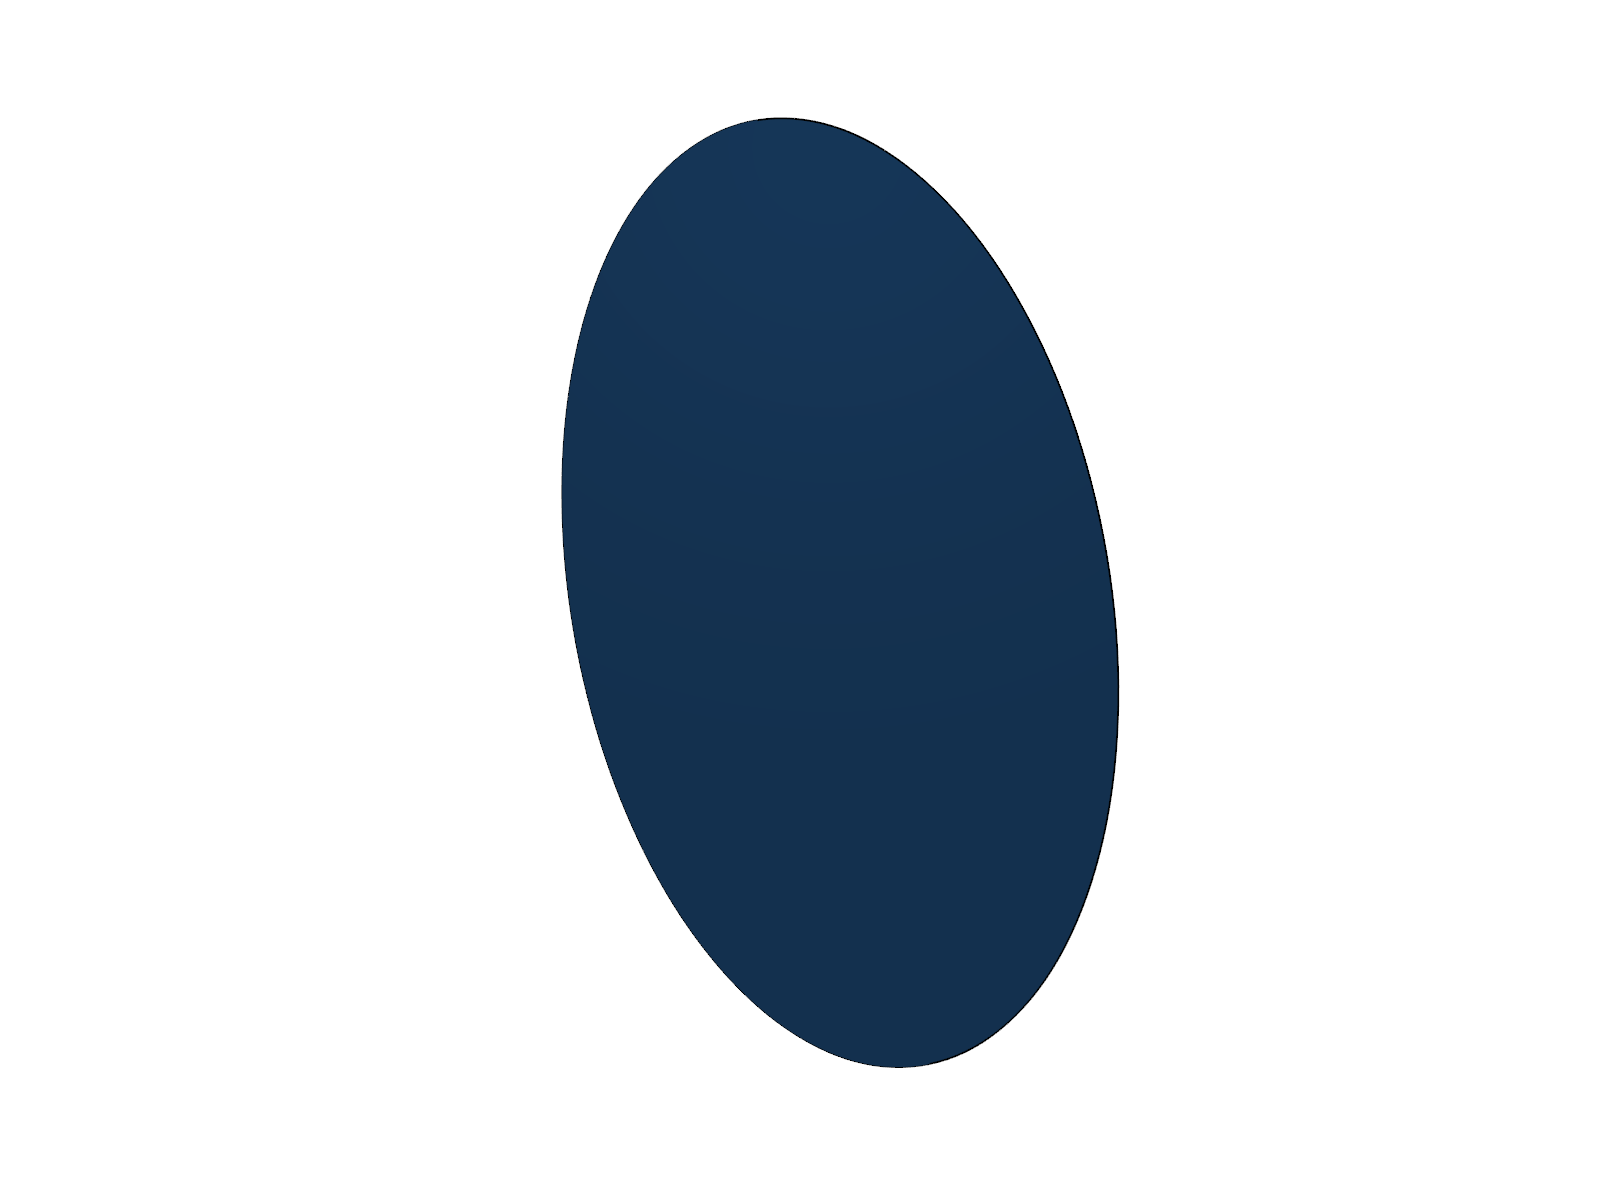
\includegraphics[width=\linewidth]{Pics/3D_inlet.png}
        \caption{Inlet}
        \label{fig:inlet3D}
    \end{subfigure}
    \hspace{0.02\textwidth}
    \begin{subfigure}[b]{0.31\textwidth}
        \centering
        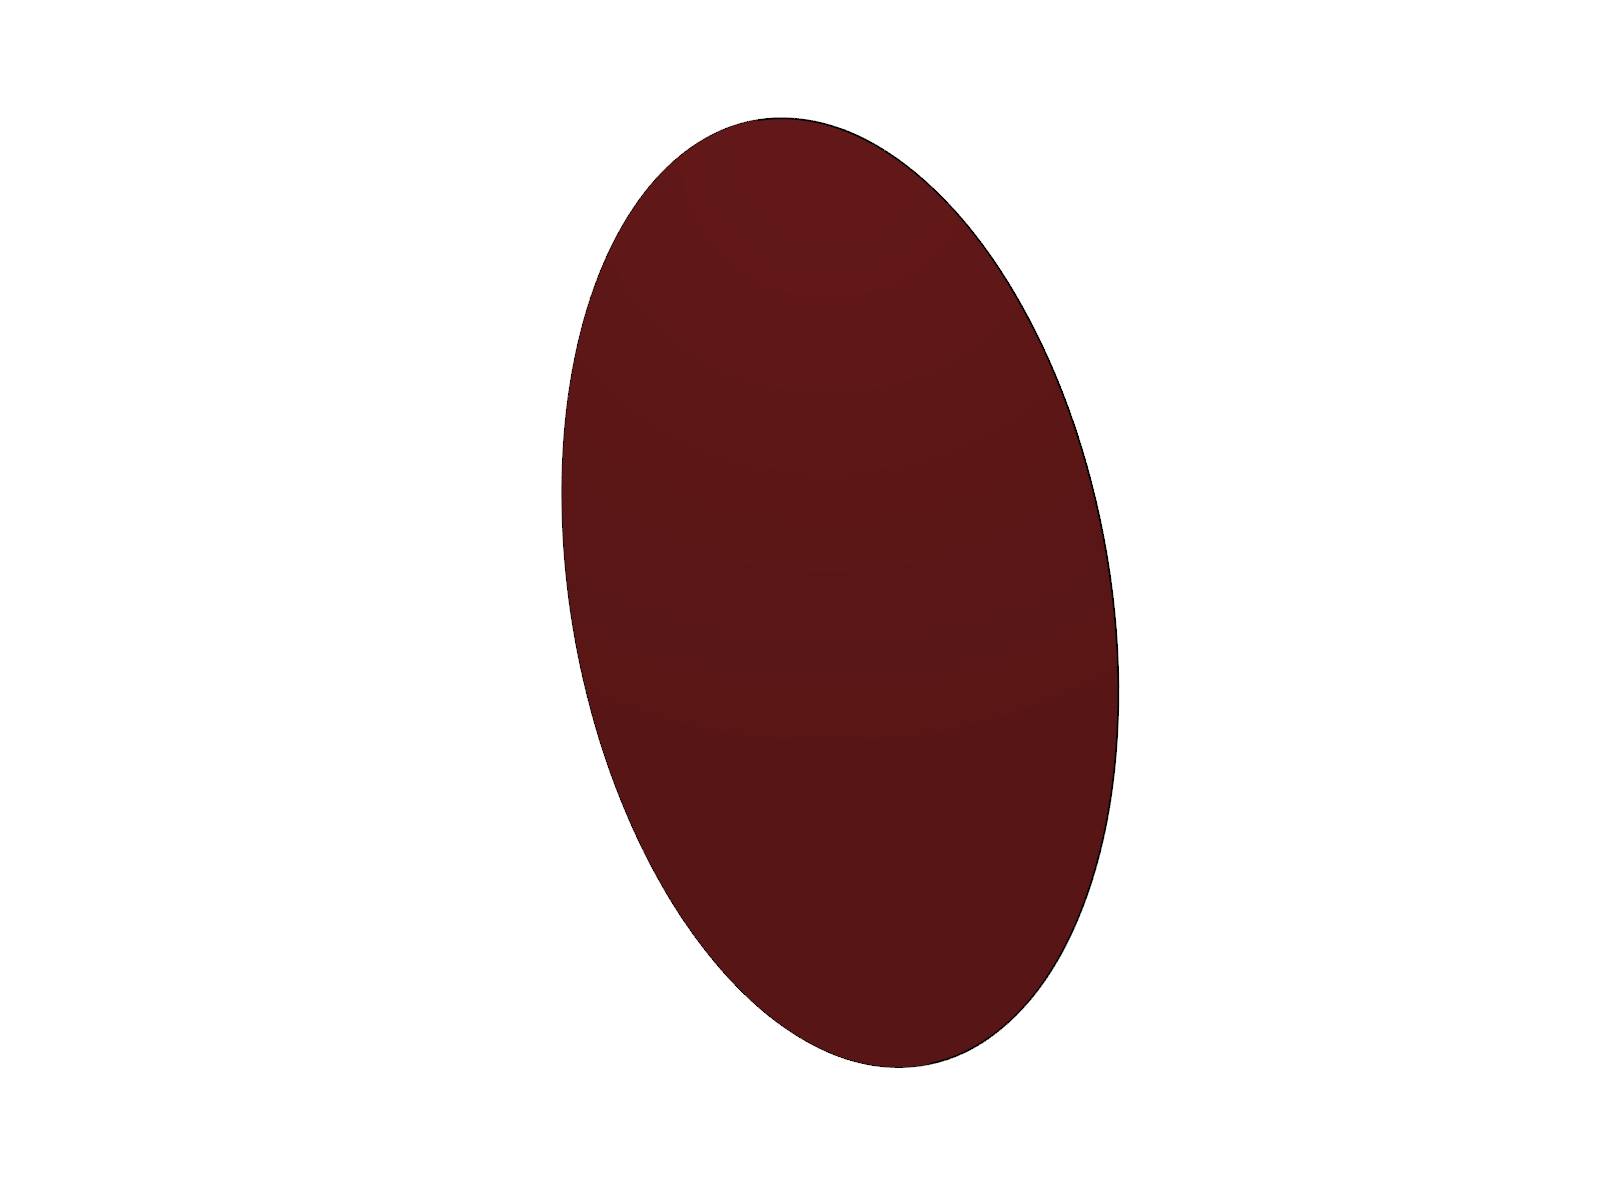
\includegraphics[width=\linewidth]{Pics/3D_outlet.png}
        \caption{Outlet}
        \label{fig:outlet3D}
    \end{subfigure}

    \vspace{0.5cm}

    % SECOND ROW: 3 images
    \begin{subfigure}[b]{0.31\textwidth}
        \centering
        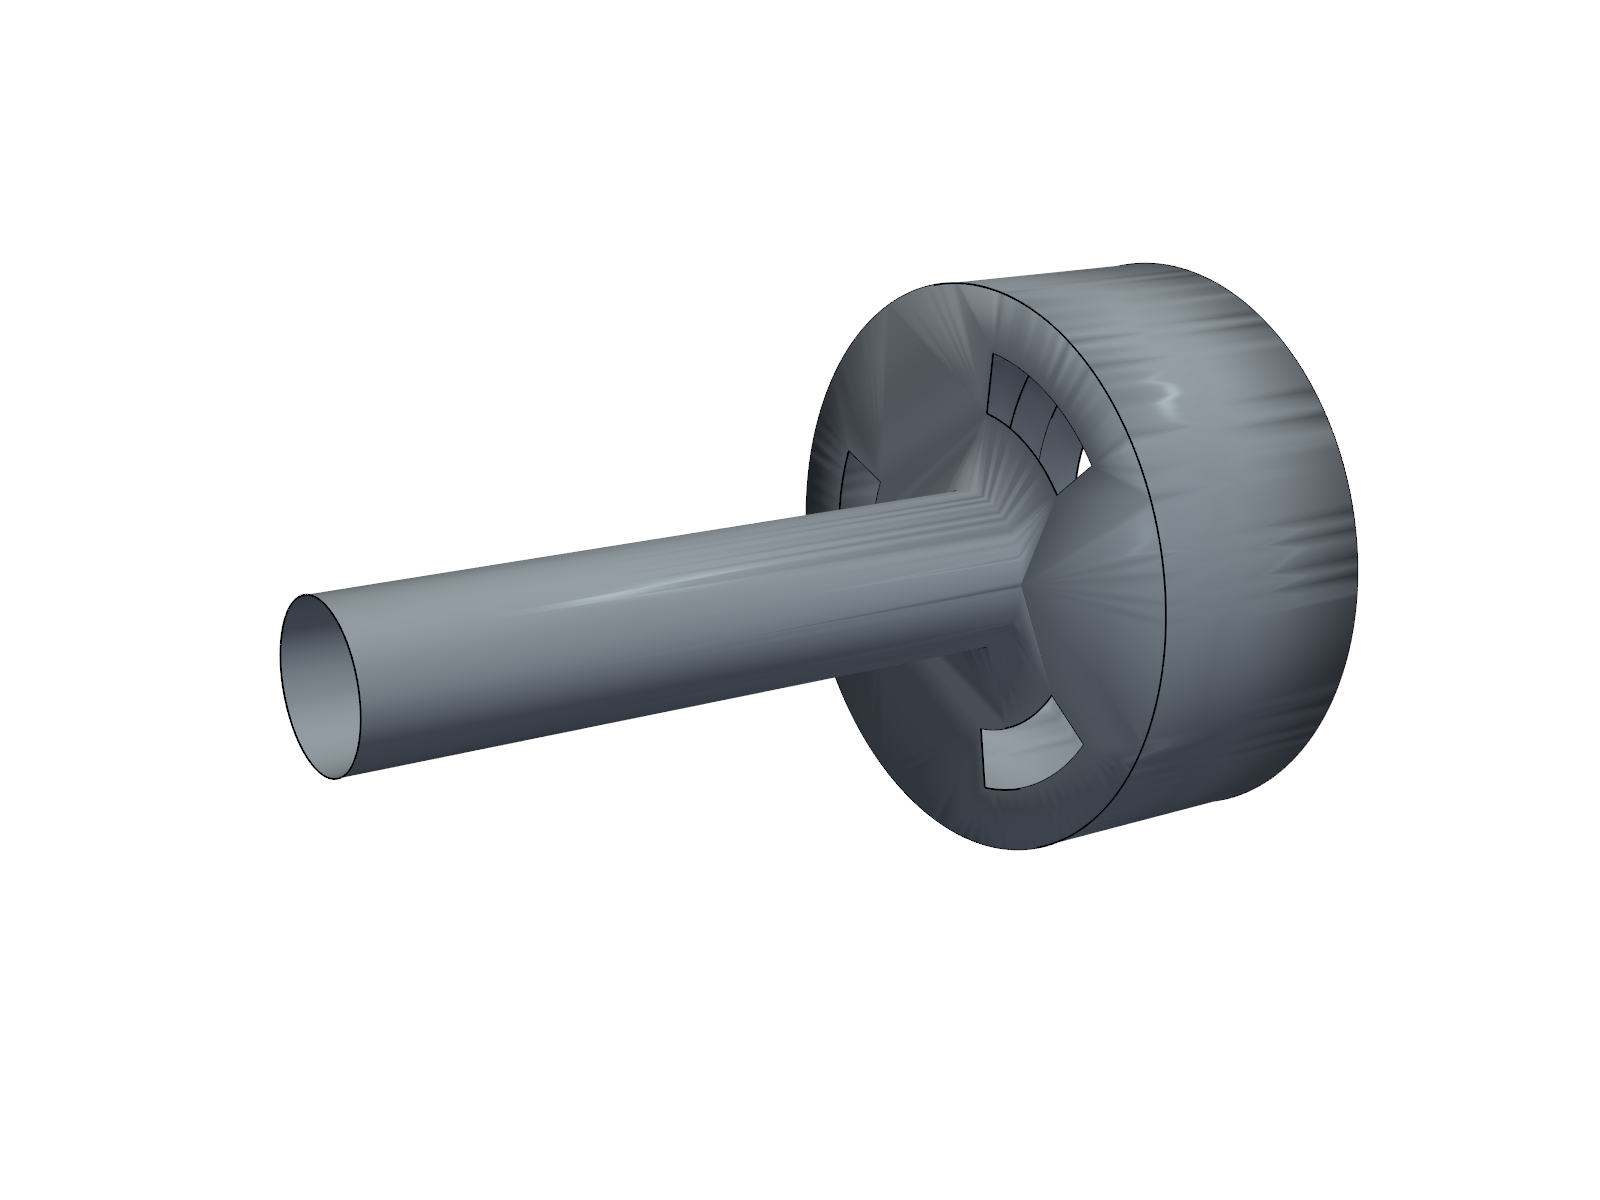
\includegraphics[width=\linewidth]{Pics/3D_wall1.png}
        \caption{Wall1}
        \label{fig:wall13D}
    \end{subfigure}
    \hfill
    \begin{subfigure}[b]{0.31\textwidth}
        \centering
        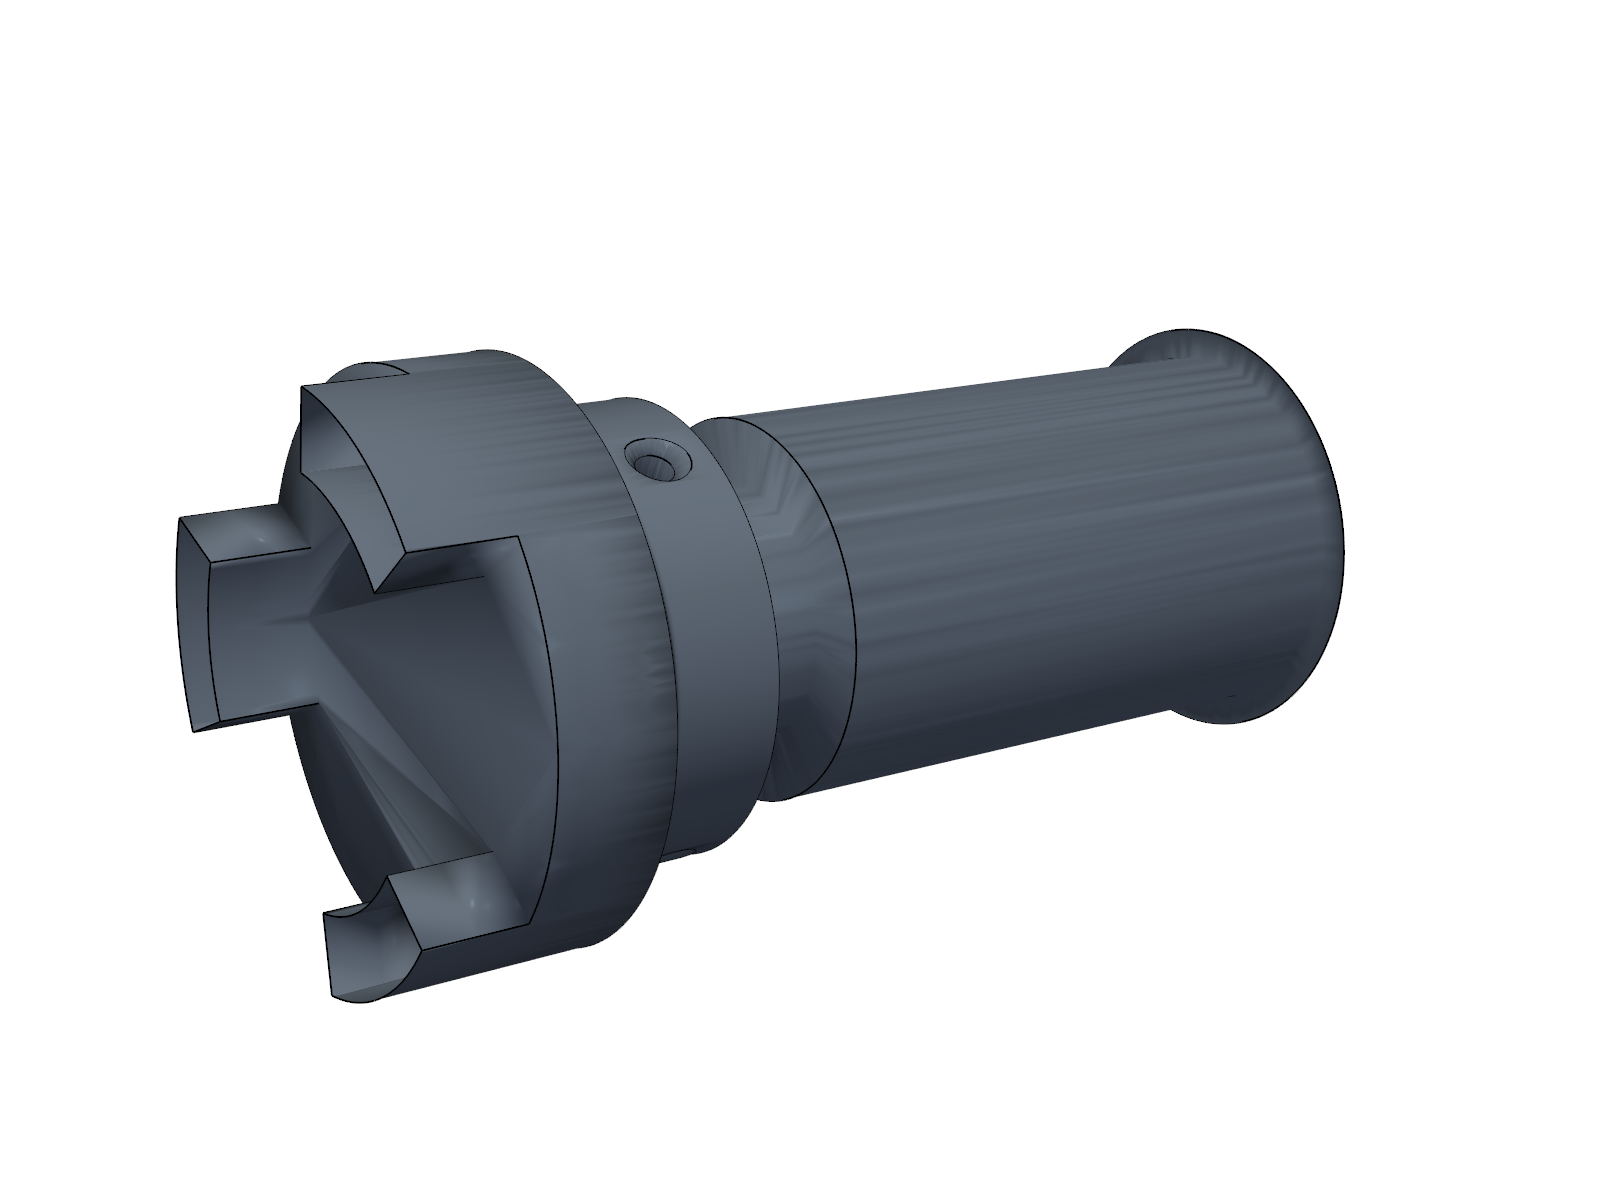
\includegraphics[width=\linewidth]{Pics/Obt_A.png}
        \caption{WallObt}
        \label{fig:wall_Obt3D}
    \end{subfigure}
    \hfill
    \begin{subfigure}[b]{0.31\textwidth}
        \centering
        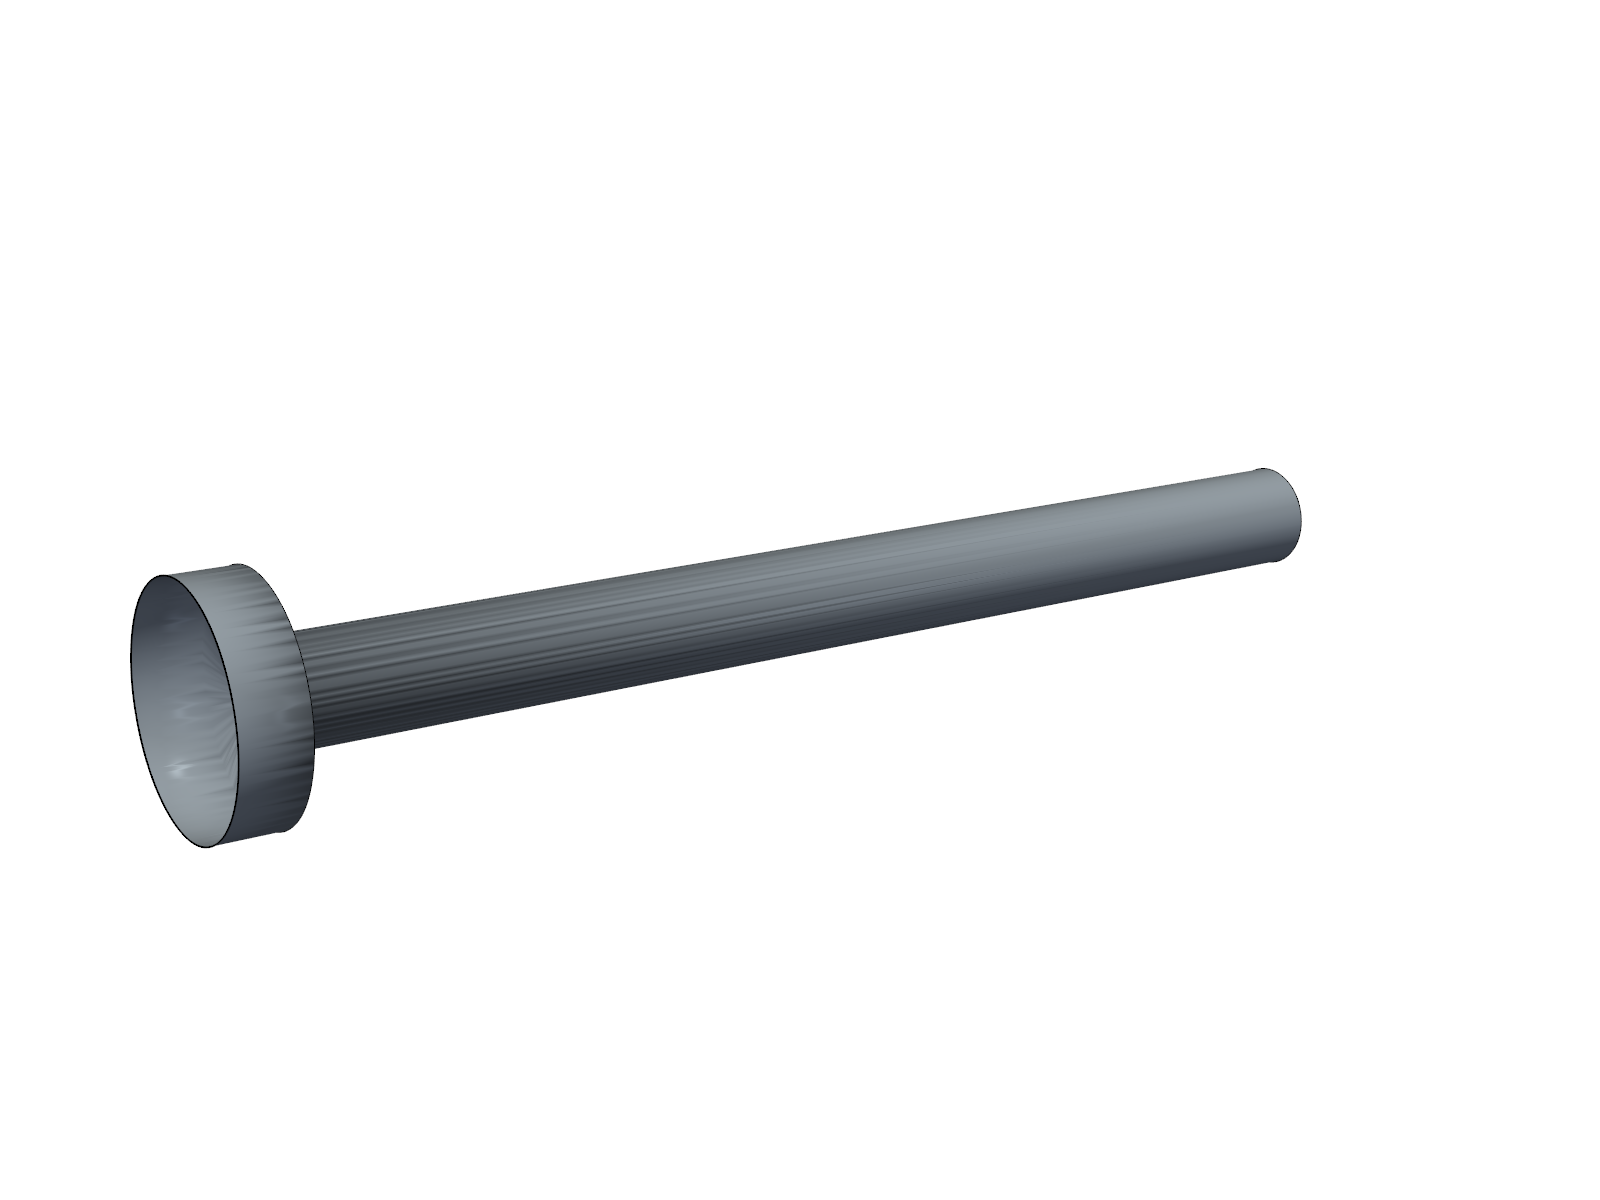
\includegraphics[width=\linewidth]{Pics/3D_wall2.png}
        \caption{Wall2}
        \label{fig:wall23D}
    \end{subfigure}

    \caption{3D overview of the numerical domain sections}
    \label{fig:Domain single sections}
\end{figure} 



\section{Workflow Automation Scripts}
\label{sec:workflow_automation}
To execute the simulations without manual intervention, a suite of Bash scripts were used, in order to manage pre-processing, solving, and directory maintenance: %

\begin{enumerate}
    \item \textbf{Full Pipeline Execution (\texttt{run\_aries\_2.sh}):} Dynamically computes the total MPI task count (\texttt{TOTAL\_TASKS=\$((SLURM\_NTASKS\_PER\_NODE * SLURM\_NNODES))}) and writes \texttt{numberOfSubdomains 52;} into \texttt{system/numProcs}, which is subsequently included via \texttt{\#include "numProcs"} inside \texttt{system/decomposeParDict}. %
    It then sequentially runs \texttt{blockMesh}, \texttt{surfaceFeatures}, \texttt{decomposePar -copyZero -force}, parallel \texttt{snappyHexMesh}, and parallel \texttt{simpleFoam}. %
    \item \textbf{Solver-Only Restart (\texttt{solver\_only.sh}):} Isolates the \texttt{mpirun -np \$TOTAL\_TASKS simpleFoam -parallel} execution, enabling rapid solver restarts or boundary condition testing without regenerating the computational grid. %
    \item \textbf{Case Maintenance (\texttt{Allclean} and \texttt{clean.sh}):} \texttt{Allclean} removes generated timestep folders (\texttt{rm -rf *[1-9]*}) and log files (\texttt{rm -f log.*}), while \texttt{clean.sh} purges the parallel processor directories (\texttt{rm -r *rocess*}). %
\end{enumerate}

\section{Hybrid Mesh Generation Strategy}
\label{sec:mesh_generation}
Spatial discretization of the fluid domain was achieved using a hybrid top-down approach that combined structured hexahedral generation with automated polyhedral surface splinting \cite{openfoam_user}. %

First, \texttt{blockMesh} constructs a structured hexahedral bounding box spanning from $(-0.01, -0.0145, -0.0145)\text{ m}$ to $(0.175, 0.0145, 0.0145)\text{ m}$, producing a total of $1,690,000$ cells, $1,746,756$ nodes and $5,126,225$ faces ($5,013,775$ internal faces), bounded by six topological patches: \texttt{front}, \texttt{back}, \texttt{inlet}, \texttt{outlet}, \texttt{bottom}, and \texttt{top}. %
The base cells exhibit nearly isotropic, orthogonal dimensions of $\Delta x = 0.4625\text{ mm}$ and $\Delta y = \Delta z = 0.4462\text{ mm}$, with an aspect ratio useful for successive refinement. %

Next, the \texttt{surfaceFeatures} utility processes the Stereolithography (\texttt{.stl}) CAD geometries defining the valve boundaries or sections as named before: \texttt{inlet.stl}, \texttt{outlet.stl}, \texttt{wall1.stl}, \texttt{wall2.stl}, and \texttt{wallObt.stl}. %
As summarized in Table \ref{tab:stl_stats}, the obturator geometry (\texttt{wallObt.stl}) presents the highest geometric complexity, comprising $10,715$ triangles and $5,637$ vertices. %
Using an included angle threshold of $150^{\circ}$, \texttt{surfaceFeatures} extracts sharp convex, concave, and region edges into \texttt{.eMesh} and \texttt{.extendedFeatureEdgeMesh} files.
Moreover, for the domain obturator section a mesh refinement regions are used in order to catch properly the flow behaviour in this domain section, which is the highest in complexity. The refinement had a \tetxttt{level \= 2} value.%
Finally, \texttt{snappyHexMesh} is executed in parallel across all cores with the \texttt{-overwrite} flag to refine cells near the feature edges, castellate the volume by removing cells outside the fluid region, and snap the boundary vertices onto the STL surfaces. %

\begin{table}[H]
\centering

\begin{tabular}{lcccc}
\toprule
\textbf{Surface File} & \textbf{Triangles} & \textbf{Vertices} & \textbf{Feature Edges} \\ %
\midrule
\texttt{inlet.stl}   & 187    & 187   & 185   \\ %
\texttt{outlet.stl}  & 187    & 187   & 185    \\ %
\texttt{wall1.stl}   & 2,990  & 1,819 & 1,819  \\ %
\texttt{wall2.stl}   & 804    & 536   & 536    \\ %
\texttt{wallObt.stl} & 10,715 & 5,637 & 2,897  \\ %
\bottomrule
\end{tabular}
\caption{Geometric statistics of the valve STL surfaces processed by \texttt{surfaceFeatures}.} %
\label{tab:stl_stats}
\end{table}

\section{HPC Infrastructure and Domain Decomposition}
\label{sec:hpc_environment}
Given the high computational cost associated with resolving the three-dimensional turbulent flow across 24 geometric and operational configurations, all numerical simulations were executed on the ARIES High-Performance Computing (HPC) cluster provided by the University of Modena and Reggio Emilia \cite{hpc_aries}. %
Job scheduling and hardware allocation were managed through the SLURM (Simple Linux Utility for Resource Management) workload manager. %

Each simulation was granted exclusive access (\texttt{--exclusive}) to a single computational node (\texttt{nodes=1}) equipped with 52 logical CPU cores (\texttt{ntasks-per-node=52}) and 490 GB of system RAM (\texttt{mem=490g}). %

Distributed memory parallelism was initialized by loading the GNU Compiler Collection (\texttt{gcc-12.1.1/gcc}) and the OpenMPI message-passing library compiled with NCCL support (\texttt{gcc-12.1.1/ompi-4.1.5\_nccl}), followed by sourcing the OpenFOAM environment configuration. %

To leverage the 52 logical processors on the ARIES node, the computational domain is partitioned prior to running \texttt{snappyHexMesh} using \texttt{decomposePar -copyZero -force}. %
The \texttt{scotch} decomposition algorithm \cite{pellegrini1996} was selected due to its ability to minimize inter-processor communication boundaries (processor faces) on complex unstructured topologies without requiring geometric directional inputs. %

The decomposition log confirms a balanced load across the 52 subdomains (\texttt{Processor 0} through \texttt{Processor 51}): %
\begin{itemize}
    \item \textbf{Average cell count per core:} $32,500$ cells. %
    \item \textbf{Maximum cell count per core:} $32,825$ cells (observed on Processors 9, 19, and 45), representing a maximum computational load imbalance of only $1\%$ above the mean. %
    \item \textbf{Inter-processor communication:} $138,841$ total processor faces, with an average of $7.69$ processor patches ($5,340$ shared faces) per core. %
\end{itemize}

%\section{Solver Configuration and Parallel Troubleshooting}
%\label{sec:solver_troubleshooting}
%Steady-state flow resolution is performed using \texttt{simpleFoam}, which implements the Semi-Implicit Method for Pressure-Linked Equations (SIMPLE) velocity-pressure coupling algorithm \cite{openfoam_user, moukalled2016}. %

%During preliminary validation runs on node \texttt{cnode05.hpc.unimo.lan}, two diagnostic behaviors were addressed in the SLURM log (\texttt{slurm-145216.out}): %
%\begin{enumerate}
 %   \item \textbf{Non-Fatal MPI/CUDA Warnings:} The OpenMPI module (\texttt{ompi-4.1.5\_nccl}) emitted warnings regarding missing shared libraries (\texttt{libcuda.so.1}) and OpenFabrics device initialization (\texttt{mlx5\_0}). %
%    Because OpenFOAM 10 executes purely on CPU cores, the absence of GPU drivers disables CUDA-aware MPI support harmlessly without impacting numerical accuracy or CPU parallel communication.
%    \item \textbf{Parallel Streamline Integer Overflow:} At the start of the time loop, the solver terminated with \texttt{FOAM FATAL ERROR: bad size -2147483647} inside \texttt{Foam::List<T>::List} (line 61 of \texttt{List.C}), triggering an \texttt{MPI\_ABORT} on rank 0. %
%    The stack trace isolated the fault to \texttt{Foam::functionObjects::streamlines::write()}. %
%    In heavily partitioned meshes (52 subdomains), lagrangian particle tracking for on-the-fly streamline generation can fail when seed points intersect processor patch boundaries, causing memory allocation counters to overflow the signed 32-bit integer limit ($-2^{31} + 1 = -2,147,483,647$). %
%    Disabling the \texttt{streamlines} function object in \texttt{system/controlDict} and deferring 3D flow visualization to offline ParaView post-processing permanently resolved the crash.
%\end{enumerate}